%\documentclass[presentation, smaller, xcolor=table]{beamer}
\documentclass[handout, smaller, xcolor=table]{beamer}			% Suppresses pauses
%\mode<handout>{\setbeamercolor{background canvas}{bg=black!5}}	% very light gray background

\usepackage{pgfpages}
	%\pgfpagesuselayout{resize to}[a4paper, border shrink=5mm, landscape]
	\pgfpagesuselayout{2 on 1}[a4paper, border shrink=5mm]		%[, portrait]
	%\pgfpagesuselayout{4 on 1}[a4paper, border shrink=5mm, landscape]
	
%\setbeameroption{show slides}
\setbeameroption{show notes}
%\setbeameroption{show only notes}

%%=========================================================================================%%
%% Themes
\usetheme{CambridgeUS}					%AnnArbor, CambridgeUS, Copenhagen, Madrid
\useoutertheme[compress, subsection=false]{miniframes}	%, footline=authorinstitutetitle
\setbeamertemplate{navigation symbols}{}		% Suppress navigation symbols in footer
%\usecolortheme{whale}

\usefonttheme[onlymath]{serif}			% To properly render mathematical symbols
%\usefonttheme[onlylarge]{structurebold}	

\setbeamercolor*{itemize item}{fg=darkred}
\setbeamertemplate{itemize item}[square]
\setbeamercolor*{itemize subitem}{fg=darkred}
\setbeamertemplate{itemize subitem}[circle]

% \usepackage{beamerthemesplit}		% Activate for custom appearance

%\setbeamertemplate{headline}[default]
%\setbeamercolor{footlinecolor}{fg=white,bg=blue}%{whale}%
%\setbeamertemplate{footline}
%{
%	\begin{beamercolorbox}[wd=\paperwidth,ht=4.0ex,dp=1.0ex,leftskip=0cm,rightskip=0cm,sep=1em]{titlelike}
%	\vspace{-2.0ex}
%	\insertshortinstitute
%	\hfill \insertshorttitle
%	\hfill \insertframenumber\,/\,\inserttotalframenumber 
%	%\hspace{0.5cm}
%	\end{beamercolorbox}
%}
%\setbeamertemplate{sidebar right}
%{
%	\vskip10pt \insertshorttitle[width={2.0cm}, center, respectlinebreaks]
%	\vskip10pt \insertshortauthor[width={2.0cm}, center]
%	\vskip10pt \insertshortinstitute[width={2.0cm}, center]
%	\vfill \hspace{0.6cm} slide \insertframenumber \ / \inserttotalframenumber
%	\vskip10pt
%}

%%=========================================================================================%%
\usepackage{layouts}	% Determines page layout specifications

\usepackage{etex}		% Resolves '/supp-pdf-mkii:137: No room for new \dimen' problem

%\usepackage[usenames,dvipsnames,table]{xcolor}	%Set option in documentclass to avoid conflict
\usepackage{graphicx}
\usepackage{epstopdf}
	\DeclareGraphicsRule{.tif}{png}{.png}{`convert #1 `dirname #1`/`basename #1 .tif`.png}

\usepackage{amsfonts, amsmath, amssymb, amsthm}
\usepackage{mathtools}
\usepackage{bbm, dsfont, mathrsfs}	
\usepackage{array, booktabs, multirow}
\usepackage[retainorgcmds]{IEEEtrantools}	%IEEEeqnarray environment
\usepackage{enumerate}

\setbeamertemplate{caption}{\insertcaption}
\setbeamerfont{caption}{size=\tiny}
%\usepackage[labelformat=empty]{caption}			%\caption*{}
%	\captionsetup[figure}{labelformat=empty}

%%=========================================================================================%%
%% Bibliography
\usepackage[numbers]{natbib}

%%=========================================================================================%%
%\theoremstyle{plain}
%\newtheorem{proposition}[theorem]{Proposition}
%
%%=========================================================================================%%
%\newcommand{\One}[1]{\mathds{1}_{\{#1\}}}
%\newcommand{\Corr}[2]{\operatorname{Corr}\!\left(#1, #2\right)}
%\newcommand{\Cov}[2]{\operatorname{Cov}\!\left(#1, #2\right)}
%\newcommand{\dee}[1]{\operatorname{d}\!#1}
%\newcommand{\Dom}[1]{\operatorname{Dom}\!#1}
%\newcommand{\normdist}[2]{\mathcal{N}\!\left(#1, #2\right)}
%\newcommand{\Ran}[1]{\operatorname{Ran}\!#1}
%\newcommand{\sgn}[1]{\operatorname{sgn}\!\left(#1\right)}
%\newcommand{\sqrts}[2][]{\,\sqrt[#1]{#2}\,}
%\newcommand{\Var}[1]{\operatorname{Var}\!\left(#1\right)}
%\newcommand{\VaR}[2][]{\operatorname{VaR}_{#1}\!\left(#2\right)}
%
%%=========================================================================================%%
\newcommand{\sqrts}[2][]{\,\sqrt[#1]{#2}\,}

\def\E{\mathbb{E}}
\def\el{l}
\def\given{\,|\,}
\def\I{\mathbb{I}}
\def\N{\mathbb{N}}
\def\one{\mathds{1}}
\def\P{\mathbb{P}}
\def\R{\mathbb{R}}
\def\S{\mathbb{S}}

\def\mwmwh{\delta}
\def\eff{\eta}

\newlength{\wherewidth}
	\settowidth{\wherewidth}{where\hspace{1em}}
\newlength{\letwidth}
	\settowidth{\letwidth}{Let\hspace{1em}}

%%=========================================================================================%%
\title[ACEMS \& CET, The University of Adelaide]{Wind Power Dispatch with Battery Energy Storage}
\subtitle{Virtual Trials in South Australia}
\author[S. Tarca et al.]{\textbf{Silvio Tarca}\inst{a} \and Matthew Roughan\inst{a} \and Nesimi Ertugrul\inst{b} \and Nigel Bean\inst{a} }
\institute[]{
	\inst{a}
	School of Mathematical Sciences and\\
	ARC Centre of Excellence for Mathematical \& Statistical Frontiers\\
	The University of Adelaide, South Australia 5005
	\and
	\inst{b}
	School of Electrical \& Electronic Engineering and\\
	Centre for Energy Technology\\
	The University of Adelaide, South Australia 5005
	\and
	\texttt{silvio.tarca@adelaide.edu.au}\\
}	
\date[December 2016]{International Conference on Energy \& Power\\RMIT University, Melbourne\\December 14--16, 2016}
\subject{}


\begin{document}

\setlength{\unitlength}{1.0mm}		% \textwidth-by-textheight is 120 mm x 90 mm
\usebackgroundtemplate{
	\begin{picture}(120,90)(0,0)	% (x,y) is 120 mm x 90 mm
		\put(0,0){\includegraphics[height=0.20\textheight]{logo_acems.jpg}}
		\put(100,0){\includegraphics[height=0.20\textheight]{logo_uofa.jpg}}
	\end{picture}
}

\begin{frame}[plain]
%% Get page layout specifications
%	The textwidth is \printinunitsof{pt}\prntlen{\textwidth} which is also \printinunitsof{in}\prntlen{\textwidth} or \printinunitsof{mm}\prntlen{\textwidth}.\\
%	The textheight is \printinunitsof{pt}\prntlen{\textheight} which is also \printinunitsof{in}\prntlen{\textheight} or \printinunitsof{mm}\prntlen{\textheight}.\\
%	The paperwidth is \printinunitsof{pt}\prntlen{\paperwidth} which is also \printinunitsof{in}\prntlen{\paperwidth} or \printinunitsof{mm}\prntlen{\paperwidth}.\\
%	The paperheight is \printinunitsof{pt}\prntlen{\paperheight} which is also \printinunitsof{in}\prntlen{\paperheight} or \printinunitsof{mm}\prntlen{\paperheight}.

	\maketitle
	
\note[item]{
This research has been undertaken jointly with Matt Roughan, Nesimi Ertugrul and Nigel Bean
}
\note[item]{
It is funded by the ARC Centre of Excellence for Mathematical \& Statistical Frontiers and the Centre for Energy Technology at The University of Adelaide 
}	
\end{frame}
\usebackgroundtemplate{}

%%=========================================================================================%%
\begin{frame}
	\frametitle{\large Registered capacity and electricity generated in SA (2015--16)}
	\framesubtitle{High penetration of intermittent renewable energy}

\note[item]{
We begin with some statistics on electricity generation in SA
}	
\begin{figure}[!h]
	\begin{minipage}{0.50\linewidth}
		\centering
		\vspace{-5pt}
		\scalebox{0.20}{
			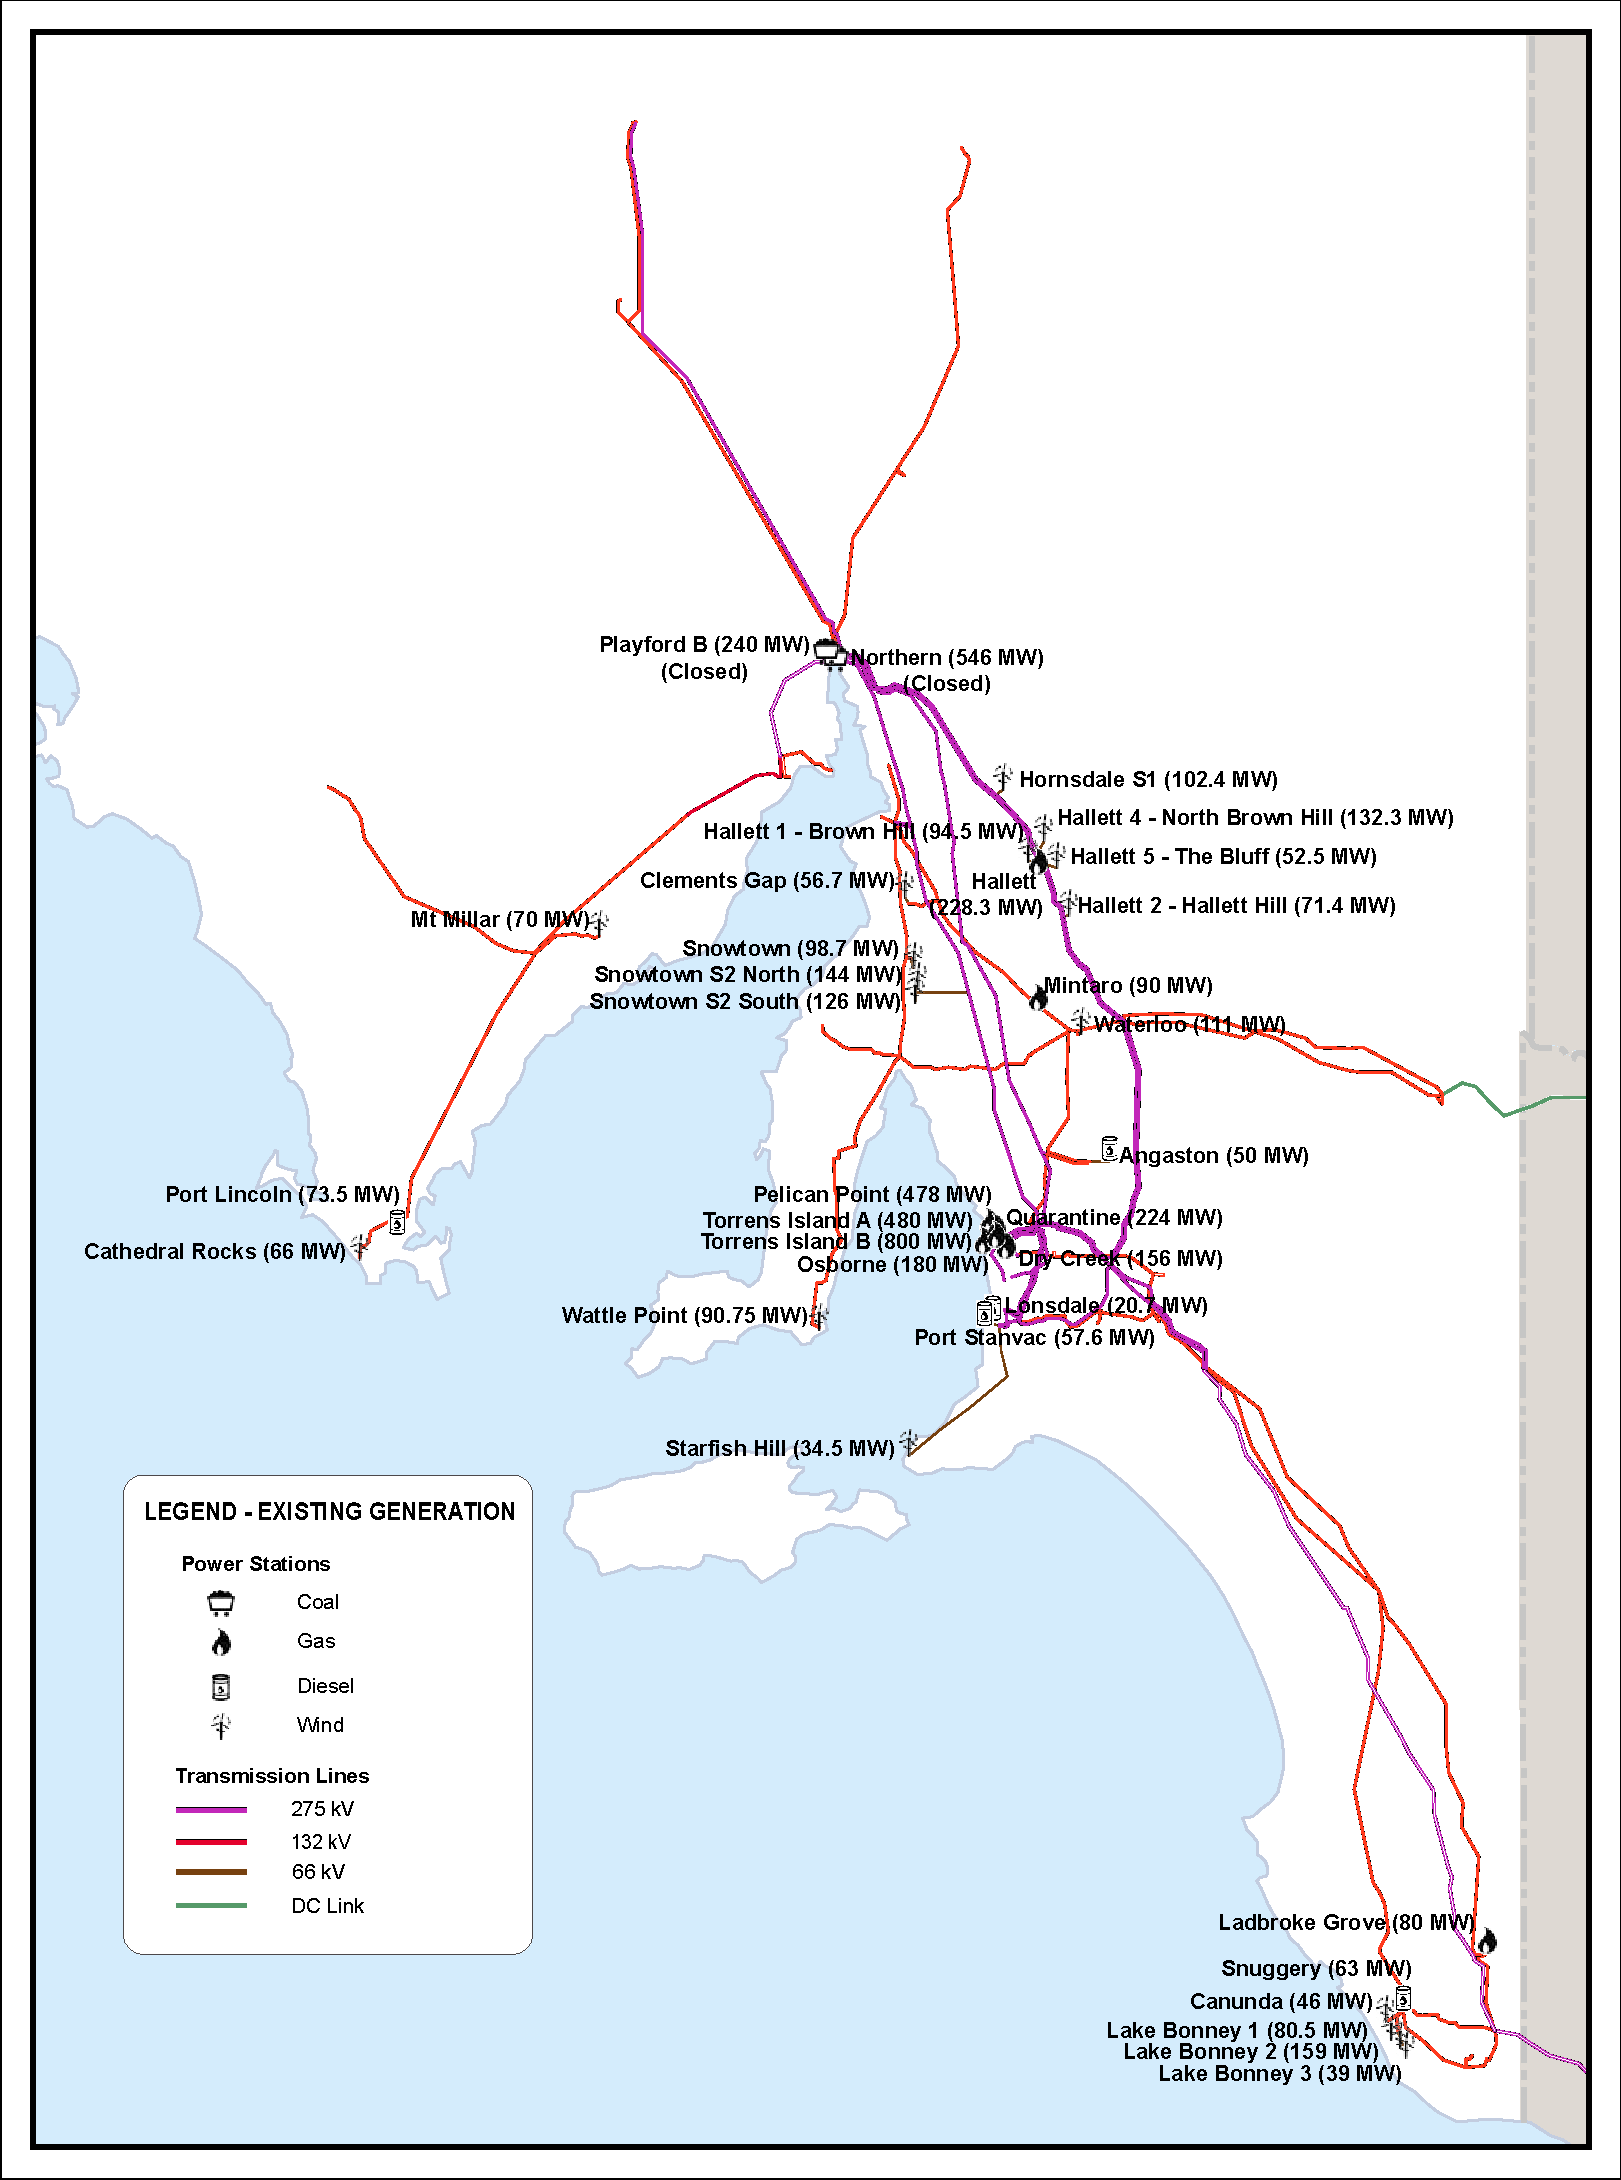
\includegraphics{sa_oper_gen_map.pdf}
		}
	\end{minipage}% To remove space between minipages
	\begin{minipage}{0.50\linewidth}
		\begin{table}[!h]
		\centering
		\label{tbl:sa_reg_cap_elec_gen}
		\scalebox{0.70}{
			\begin{tabular}{l r r r r}
			\toprule
			Energy	& \multicolumn{2}{c}{Registered capacity}	& \multicolumn{2}{c}{Electricity generated} \\
			source	& \multicolumn{1}{c}{MW}	& \multicolumn{1}{c}{\% of total}	&  \multicolumn{1}{c}{GWh}	& \multicolumn{1}{c}{\% of total}	\\
			\midrule
			Gas			& 2,668	& 44.6	& 4,538	& 36.4	\\
			Wind			& 1,576	& 26.3	& 4,322	& 34.7	\\
			Coal			& 770	& 12.9	& 2,601	& 20.9	\\
			Rooftop PV	& 679	& 11.4	& 938	& 7.5		\\
			Other		& 289	& 4.8		& 60		& 0.5		\\
			\midrule
			Total			& 5,982	& 100.0	& 12,459	& 100.0	\\
			\bottomrule
			\end{tabular}	
    		}
		\caption{Source: Australian Energy Market Operator}
		\end{table}
		
		{\footnotesize Following the closure of the last coal-fired power plant in SA, from 10 May 2016 to 31 July 2016, 51\% of electricity generated in the state came from wind and rooftop PV\par}
	\end{minipage}
\end{figure}

\end{frame}

%%=========================================================================================%%
\begin{frame}
	\frametitle{Market and security challenges faced by SA}
	\framesubtitle{}

\note[item]{
This generation mix presents market and engineering challenges for SA including \ldots
}	
	\begin{itemize}
		\item  Dependable supply of scheduled (baseload) power:
		\begin{itemize}
			\item  High penetration of intermittent renewable energy
			\item  Limited connectivity with other regions in the NEM
\note[item]{
SA is at the end of a long, skinny transmission network that constitutes NEM
}
		\end{itemize}
		\item  High and volatile wholesale electricity prices:
		\begin{itemize}
			\item  Variability in wind and solar power generation
			\item  Difficulty in making wind and solar forecasts, especially about the future
			\item  Balance of generation is gas-fired
\note[item]{
Expanding market for Australian LNG exports is driving domestic wholesale gas prices to international parity, so now we're experiencing historically high domestic gas prices
}			
		\end{itemize}
		\item  Secure operation of the power system:
\note[item]{
Note that in power engineering \textit{secuirty} refers to `keeping the lights on', not cyber-attacks
}
		\begin{itemize}
			\item  Ancillary services historically provided by conventional synchronous generators
\note[item]{
Conventional generators --- voltage is synchronised with the rotor position and frequency depends on the rotor speed
}
			\item  Renewable energy generation is displacing conventional generation as SA transitions to a low-carbon economy 
			\item  Tight availability of locally provisioned ancillary services when islanded
\note[item]{
Particularly problematic in the event of loss of the Heywood Interconnector resulting in SA separation from the rest of NEM
}			
		\end{itemize}
	\end{itemize}

\end{frame}

%%=========================================================================================%%
\begin{frame}
	\frametitle{Wind power dispatch with battery energy storage}
	\framesubtitle{State-space model predictive control (MPC)}

	\hspace{-1.5em}
	\begin{minipage}{0.57\linewidth}
\note[item]{
This paper is concerned with the challenge of supplying baseload power from an SA wind farm, and to facilitate the supply of baseload power we suppose that a utility-scale battery has been coupled to the wind farm, enabling time shifting of wind power dispatched to the grid
}
		\begin{itemize}
			\item  Suppose that a utility-scale battery has been coupled to an SA wind farm
			\item  Represent the process of wind power dispatch with battery energy storage as a state-space model
\note[item]{
State-space model describes process outputs as a function of state variables which depend on control signals
}
			\item  MPC controller computes battery charge/ discharge control signals by minimising tracking error of power dispatched to the grid relative to a set point --- target baseload power
\note[item]{
Use model predictive control to optimise battery charge/discharge control signals with the objective of minimising tracking error
}
			\item	 Virtual trials measure the improvement in dispatchability of wind power with battery energy storage
\note[item]{
Virtual trial: computer simulation using real-world data
}
		\end{itemize}
	\end{minipage}% To remove space between minipages
	\begin{minipage}{0.43\linewidth}
		\scalebox{0.269}{
			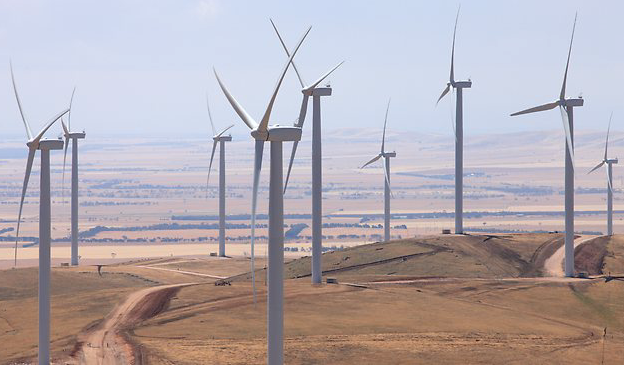
\includegraphics{wind_farm.png}
		}
		\scalebox{0.169}{
			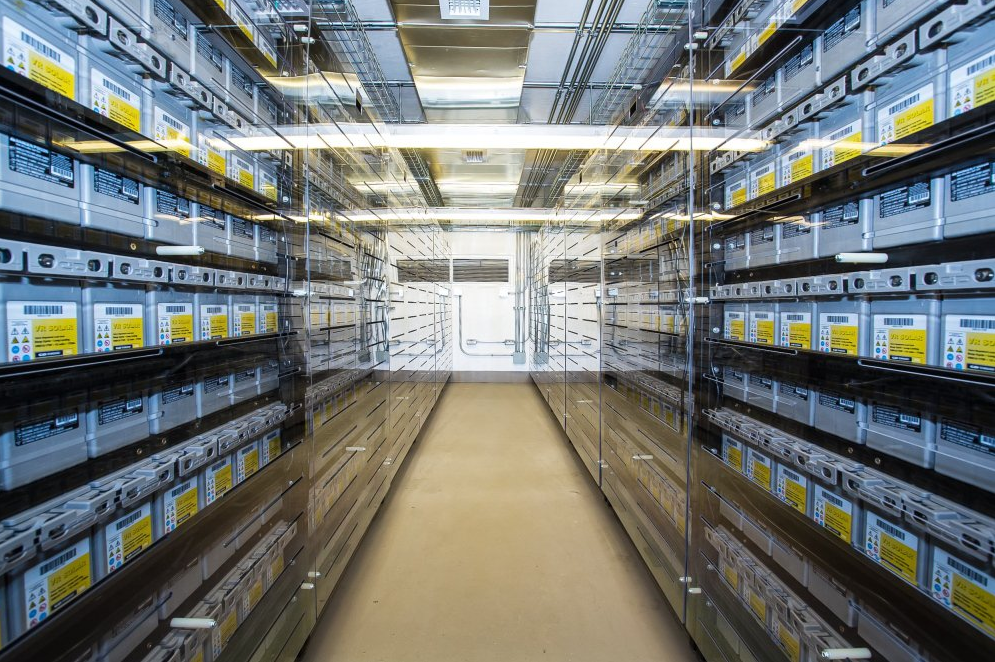
\includegraphics{battery.png}
    		}
	\end{minipage}

\end{frame}

%%=========================================================================================%%
\begin{frame}
	\frametitle{Modelling contributions to the literature}
	\framesubtitle{Proper accounting of battery charge/discharge efficiency}
	
\note[item]{
In relation to the process of wind power dispatch with battery energy storage, we highlight a couple of contributions to the literature
} 
\note[item]{
Firstly, we properly account for battery charge/discharge efficiency, denoted by $\eta$, in the first equation describing the time evolution of SOC of the battery
}
\note[item]{
Prior papers either assume 100\% efficiency, or approximate energy loss independent of the power stored or discharged during the dispatch interval
}
\note[item]{
Observe that the factor $\mwmwh$ converts power (MW) supplied to, or discharged from, the battery over the dispatch interval to energy (MWh).  It follows that the conversion factor for a 5-minute dispatch interval is $\mwmwh = \tfrac{1}{12}$
}
\note[item]{
In the second equation power dispatched to the grid is equal to wind power plus power discharged from the battery minus power diverted from the grid to charge the battery
} 
	\vspace{1.0em}
	Time evolution of state of charge (SOC) of the battery,
	\begin{IEEEeqnarray*}{rCl}
		e(t\!+\!1) & = & e(t) + {\mwmwh\eff}p_{b+}(t) -  \frac{\mwmwh}{\eff}p_{b-}(t)	,
	\end{IEEEeqnarray*}
	properly accounts for battery charge/discharge efficiency, and\\power dispatched to the grid is given by
	\begin{IEEEeqnarray*}{rCl}
		p_{d}(t\!+\!1) & = & p_{b-}(t) - p_{b+}(t) + p_{w}(t),
	\end{IEEEeqnarray*}
	where\hspace{1em}${p_{b+}(t) \geq 0}$ is the battery charge control signal,	\\
	\hspace{\wherewidth}${p_{b-}(t) \geq 0}$ the battery discharge control signal,	\\
	\hspace{\wherewidth}${p_{w}(t) \geq 0}$ the wind power control signal, \\
	\hspace{\wherewidth}${\eff\in(0,1]}$ the one-way charge/discharge efficiency of the battery, and\\
	\hspace{\wherewidth}${\mwmwh > 0}$ the conversion factor from MW to MWh for the dispatch interval

\end{frame}

%%=========================================================================================%%
\begin{frame}
	\frametitle{Modelling contributions to the literature}
	\framesubtitle{Incremental state-space model}

\note[item]{
Our second contribution to the literature is to represent the process of wind power dispatch with battery energy storage as an incremental state-space model, which allows that MPC controller to penalise control effort
}
	Incremental formulation of the state-space model for wind power dispatch with battery energy storage allows the MPC controller to penalise control effort
	\note[item]{
Control effort is captured by the control increment vector $\boldsymbol{\Delta{u}}(t)$, i.e., the vector of changes in battery charge, battery discharge and wind power control signals
}
\note[item]{
The first matrix equation describes the time evolution of state variables, $\boldsymbol{z}(t)$, which depend on control increments, $\boldsymbol{\Delta{u}}(t)$
}
\note[item]{
Observe that in the incremental formulation of the state-space model, control signals, ${\boldsymbol{u}(t) = \begin{bmatrix*}[c] p_{b+}(t) & p_{b-}(t) & p_{w}(t) \end{bmatrix*}^{T}}$, become internal state variables augmenting observable state variables, $e(t)$, and control increments, ${\boldsymbol{\Delta{u}}(t) = \begin{bmatrix*}[c] \Delta{p_{b+}}(t) & \Delta{p_{b-}}(t) & \Delta{p_{w}}(t) \end{bmatrix*}^{T}}$, serve as process inputs
}
\note[item]{
The second matrix equation maps state variables, $\boldsymbol{z}(t\!+\!1)$, to process outputs, ${\boldsymbol{y}(t\!+\!1) = \begin{bmatrix*}[c] e(t\!+\!1) & p_{d}(t\!+\!1) \end{bmatrix*}^{T}}$, where $A$, $B$ and $C$ are matrices defining the single-period, incremental state-space model
}
\note[item]{
Notice that for an abstract process in steady state the control increment required to maintain zero tracking error of a process output relative to its set point is zero
}
		
	\begin{IEEEeqnarray*}{rCl}
            	% State matrix equation for electricity dispatch
            	\underset{\boldsymbol{z}(t+1)}{
            	\begin{bmatrix*}[c]
            		e(t\!+\!1)	\\
            		p_{b+}(t)	\\
            		p_{b-}(t)	\\
            		p_{w}(t)	\\
            	\end{bmatrix*}}
            	& = &
            	\underset{A}{
            	\begin{bmatrix*}[c]
            		1	& \mwmwh\eff	& -\mwmwh/\eff	& 0	\\
            		0	& 1			& 0			& 0	\\
            		0	& 0			& 1			& 0	\\
            		0	& 0			& 0			& 1	\\
                	\end{bmatrix*}}
            	\underset{\boldsymbol{z}(t)}{
            	\begin{bmatrix*}[c]
            		e(t)	\\
            		p_{b+}(t\!-\!1)	\\
            		p_{b-}(t\!-\!1)	\\
            		p_{w}(t\!-\!1)	\\
            	\end{bmatrix*}}
            	+
            	\underset{B}{
            	\begin{bmatrix*}[c]
            		\mwmwh\eff	& -\mwmwh/\eff	& 0	\\
            		1			& 0			& 0	\\
            		0			& 1			& 0	\\
            		0			& 0			& 1	\\
            	\end{bmatrix*}}
            	\underset{\boldsymbol{\Delta{u}}(t)}{
            	\begin{bmatrix*}[c]
            		\Delta{p_{b+}}(t)	\\
            		\Delta{p_{b-}}(t)		\\
            		\Delta{p_{w}}(t)		\\
            	\end{bmatrix*}},		\\[10pt]
            	% Process output matrix equation for electricity dispatch
            	\underset{\boldsymbol{y}(t+1)}{
            	\begin{bmatrix*}[c]
            		e(t\!+\!1)		\\
            		p_{d}(t\!+\!1)	\\
            	\end{bmatrix*}}
            	& = &
            	\underset{C}{
            	\begin{bmatrix*}[c]
            		1	& 0	& 0	& 0	\\
            		0	& -1	& 1	& 1	\\
            	\end{bmatrix*}}
            	\underset{\boldsymbol{z}(t+1)}{
            	\begin{bmatrix*}[c]
            		e(t\!+\!1)	\\
            		p_{b+}(t)	\\
            		p_{b-}(t)	\\
            		p_{w}(t)	\\
                	\end{bmatrix*}}
	\end{IEEEeqnarray*}
	
\end{frame}

%%=========================================================================================%%
\begin{frame}
	\frametitle{Optimisation of the performance index}
	\framesubtitle{}
	
	MPC controller determines control increments by optimising a performance index that penalises tracking error and control effort
\note[item]{
Tracking error is defined as the Euclidean norm of the difference between predicted process outputs and their respective set points, while control effort is defined as the Euclidean norm of control increments
}
\note[item]{
Squaring both tracking error and control effort, and multiplying by weighting coefficients ($\lambda$, $\Omega$ and $\Psi$)yields the quadratic cost (or objective) function $f$
}
\note[item]{
Then, expanding the cost function, dropping the constant terms and imposing process constraints on state variables, the quadratic optimisation problem is written in standard form as presented here
}
\note[item]{
Notice that the optimiser solves for the argument $\boldsymbol{\Delta{u}}(t)$ that minimises the objective function subject to process constraints
}

	\begin{itemize}
		\item  Let $\boldsymbol{r}(t)\in\R^{m}$ be a set-point vector, and define the quadratic cost function
	\begin{IEEEeqnarray*}{rCl}
    		f & = & \left\lVert\sqrts{\Omega}\left(\boldsymbol{r}(t\!+\!1)-\boldsymbol{y}(t\!+\!1)\right)\right\rVert_{2}^{2} + \lambda\left\lVert\sqrts{\Psi}\boldsymbol{\Delta{u}}(t)\right\rVert_{2}^{2},	
	\end{IEEEeqnarray*}
where $\lambda \geq 0$ is a scalar weighting coefficient, and $\Omega\in\R^{m\times{m}}$ and $\Psi \in\R^{q\times{q}}$ are positive semidefinite diagonal weighting matrices
		\item  Process constraints take the form of bounds on observable and internal state variables, the latter expressed in terms of control increments
		\item  Quadratic optimisation problem is written in standard form:
	\begin{IEEEeqnarray*}{rCl}
		\underset{\boldsymbol{\Delta{u}}(t)}{\operatorname{argmin}} & \quad & 
	\frac{1}{2}\boldsymbol{\Delta{u}}(t)^{T}\left(B^{T}C^{T}\Omega{CB} + \lambda\Psi\right)\boldsymbol{\Delta{u}}(t) \\
		& & + \big(CA\boldsymbol{z}(t) - \boldsymbol{r}(t\!+\!1)\big)^{T}\Omega{CB}\boldsymbol{\Delta{u}}(t)	\\
    		\operatorname{subject\ to} & & \underline{\boldsymbol{x}} \preceq \boldsymbol{x}(t\!+\!1) \preceq \overline{\boldsymbol{x}},	\\
		& & \underline{\boldsymbol{\Delta{u}}} \preceq \boldsymbol{\Delta{u}}(t) \preceq \overline{\boldsymbol{\Delta{u}}}
	\end{IEEEeqnarray*}

	\end{itemize}

\note[item]{
To ensure linear complementarity of battery charge and discharge control signals, we reformulate optimisation problem as a mixed integer quadratic program and solve it using \texttt{cplexmiqp()} from the CPLEX for MATLAB Toolbox
}
	
\end{frame}

%%=========================================================================================%%
\begin{frame}
	\frametitle{Virtual trials in South Australia}
	\framesubtitle{}

\note[item]{
Our empirical analysis implements \ldots
}	
	\begin{itemize}
		\item  Implement a na\"ive, single-period dispatch strategy:
		\begin{itemize}
			\item  Charge battery with surplus wind power whenever available capacity for dispatch exceeds the set point
			\item  Discharge battery to supplement wind power whenever available capacity for dispatch is less than the set point
		\end{itemize}
		\item  Virtual trials perform computer simulations using real-world data:
		\begin{itemize}
			\item  Optimise control increments for 5-minute dispatch intervals from 1~April~2015 to 31~March~2016 using publicly available dispatch data
			\item  For different set points representing target baseload power
			\item  For different size utility-scale batteries
		\end{itemize}
		\item  Some observations:
		\begin{itemize}
			\item  Probability of power dispatched to the grid supplying a target baseload power is moderately higher with battery energy storage
			\item  Not very sensitive to shape of the load profile or battery charge/discharge efficiency due to autocorrelation of wind power over dispatch intervals
			\item  Even on today's utility scale, battery power can only substitute for a fraction of the registered capacity of a commercial wind farm for a limited time
		\end{itemize}  
		
	\end{itemize}
	
\end{frame}

%%=========================================================================================%%
\begin{frame}
	\frametitle{\large Improvement in Wind Power Dispatch with Battery Energy Storage}
	\framesubtitle{}

\note[item]{
We use publicly available dispatch data published by AEMO for the Snowtown wind farm in the state's mid-north.  It has a registered capacity of 100 MW, which we take as the base quantity for power in the per unit system.  And to keep it simple we choose 100 MWh as the base quantity for energy 
}
\note[item]{
On the $y$-axis is the probability of power dispatched to the grid equaling or exceeding the set point representing target baseload power, which is on the $x$-axis
}
\note[item]{
There are five curves: the bottom black solid curve is for the Snowtown wind farm with no energy storage, and the four curves above it correspond to virtual trials supposing that utility-scale batteries of increasing size are coupled to the wind farm
}
	{\footnotesize Number of 5-minute dispatch intervals over one year where power dispatched to the grid exceeds target baseload power is 10--28\% higher with a utility-scale battery than no energy storage\par}

	\begin{figure}[!h]
		\centering
    		\label{fig:disp_wind_bess}
		\scalebox{0.72}{
			% GNUPLOT: LaTeX picture with Postscript
\begingroup
  \makeatletter
  \providecommand\color[2][]{%
    \GenericError{(gnuplot) \space\space\space\@spaces}{%
      Package color not loaded in conjunction with
      terminal option `colourtext'%
    }{See the gnuplot documentation for explanation.%
    }{Either use 'blacktext' in gnuplot or load the package
      color.sty in LaTeX.}%
    \renewcommand\color[2][]{}%
  }%
  \providecommand\includegraphics[2][]{%
    \GenericError{(gnuplot) \space\space\space\@spaces}{%
      Package graphicx or graphics not loaded%
    }{See the gnuplot documentation for explanation.%
    }{The gnuplot epslatex terminal needs graphicx.sty or graphics.sty.}%
    \renewcommand\includegraphics[2][]{}%
  }%
  \providecommand\rotatebox[2]{#2}%
  \@ifundefined{ifGPcolor}{%
    \newif\ifGPcolor
    \GPcolorfalse
  }{}%
  \@ifundefined{ifGPblacktext}{%
    \newif\ifGPblacktext
    \GPblacktexttrue
  }{}%
  % define a \g@addto@macro without @ in the name:
  \let\gplgaddtomacro\g@addto@macro
  % define empty templates for all commands taking text:
  \gdef\gplbacktext{}%
  \gdef\gplfronttext{}%
  \makeatother
  \ifGPblacktext
    % no textcolor at all
    \def\colorrgb#1{}%
    \def\colorgray#1{}%
  \else
    % gray or color?
    \ifGPcolor
      \def\colorrgb#1{\color[rgb]{#1}}%
      \def\colorgray#1{\color[gray]{#1}}%
      \expandafter\def\csname LTw\endcsname{\color{white}}%
      \expandafter\def\csname LTb\endcsname{\color{black}}%
      \expandafter\def\csname LTa\endcsname{\color{black}}%
      \expandafter\def\csname LT0\endcsname{\color[rgb]{1,0,0}}%
      \expandafter\def\csname LT1\endcsname{\color[rgb]{0,1,0}}%
      \expandafter\def\csname LT2\endcsname{\color[rgb]{0,0,1}}%
      \expandafter\def\csname LT3\endcsname{\color[rgb]{1,0,1}}%
      \expandafter\def\csname LT4\endcsname{\color[rgb]{0,1,1}}%
      \expandafter\def\csname LT5\endcsname{\color[rgb]{1,1,0}}%
      \expandafter\def\csname LT6\endcsname{\color[rgb]{0,0,0}}%
      \expandafter\def\csname LT7\endcsname{\color[rgb]{1,0.3,0}}%
      \expandafter\def\csname LT8\endcsname{\color[rgb]{0.5,0.5,0.5}}%
    \else
      % gray
      \def\colorrgb#1{\color{black}}%
      \def\colorgray#1{\color[gray]{#1}}%
      \expandafter\def\csname LTw\endcsname{\color{white}}%
      \expandafter\def\csname LTb\endcsname{\color{black}}%
      \expandafter\def\csname LTa\endcsname{\color{black}}%
      \expandafter\def\csname LT0\endcsname{\color{black}}%
      \expandafter\def\csname LT1\endcsname{\color{black}}%
      \expandafter\def\csname LT2\endcsname{\color{black}}%
      \expandafter\def\csname LT3\endcsname{\color{black}}%
      \expandafter\def\csname LT4\endcsname{\color{black}}%
      \expandafter\def\csname LT5\endcsname{\color{black}}%
      \expandafter\def\csname LT6\endcsname{\color{black}}%
      \expandafter\def\csname LT7\endcsname{\color{black}}%
      \expandafter\def\csname LT8\endcsname{\color{black}}%
    \fi
  \fi
    \setlength{\unitlength}{0.0500bp}%
    \ifx\gptboxheight\undefined%
      \newlength{\gptboxheight}%
      \newlength{\gptboxwidth}%
      \newsavebox{\gptboxtext}%
    \fi%
    \setlength{\fboxrule}{0.5pt}%
    \setlength{\fboxsep}{1pt}%
\begin{picture}(8162.00,5442.00)%
    \gplgaddtomacro\gplbacktext{%
      \csname LTb\endcsname%
      \put(814,704){\makebox(0,0)[r]{\strut{}0}}%
      \put(814,1151){\makebox(0,0)[r]{\strut{}10}}%
      \put(814,1599){\makebox(0,0)[r]{\strut{}20}}%
      \put(814,2046){\makebox(0,0)[r]{\strut{}30}}%
      \put(814,2493){\makebox(0,0)[r]{\strut{}40}}%
      \put(814,2941){\makebox(0,0)[r]{\strut{}50}}%
      \put(814,3388){\makebox(0,0)[r]{\strut{}60}}%
      \put(814,3835){\makebox(0,0)[r]{\strut{}70}}%
      \put(814,4282){\makebox(0,0)[r]{\strut{}80}}%
      \put(814,4730){\makebox(0,0)[r]{\strut{}90}}%
      \put(814,5177){\makebox(0,0)[r]{\strut{}100}}%
      \put(946,484){\makebox(0,0){\strut{}0.00}}%
      \put(1855,484){\makebox(0,0){\strut{}0.10}}%
      \put(2764,484){\makebox(0,0){\strut{}0.20}}%
      \put(3674,484){\makebox(0,0){\strut{}0.30}}%
      \put(4583,484){\makebox(0,0){\strut{}0.40}}%
      \put(5492,484){\makebox(0,0){\strut{}0.50}}%
      \put(6401,484){\makebox(0,0){\strut{}0.60}}%
      \put(7310,484){\makebox(0,0){\strut{}0.70}}%
    }%
    \gplgaddtomacro\gplfronttext{%
      \csname LTb\endcsname%
      \put(176,2940){\rotatebox{-270}{\makebox(0,0){\strut{}$\P\left(\text{power dispatched} \geq \text{set point}\right)$, \%}}}%
      \put(4355,154){\makebox(0,0){\strut{}Average of set points for power dispatched to the grid, p.u.}}%
      \csname LTb\endcsname%
      \put(1894,1936){\makebox(0,0)[l]{\strut{}No energy storage}}%
      \csname LTb\endcsname%
      \put(1894,1716){\makebox(0,0)[l]{\strut{}Battery (1), energy capacity = 0.25 p.u.}}%
      \csname LTb\endcsname%
      \put(1894,1496){\makebox(0,0)[l]{\strut{}Battery (2), 0.50 p.u.}}%
      \csname LTb\endcsname%
      \put(1894,1276){\makebox(0,0)[l]{\strut{}Battery (3), 0.75 p.u.}}%
      \csname LTb\endcsname%
      \put(1894,1056){\makebox(0,0)[l]{\strut{}Battery (4), 1.00 p.u.}}%
      \csname LTb\endcsname%
      \put(4846,4506){\makebox(0,0)[l]{\strut{}Capacity factor = 0.38}}%
      \put(4846,4730){\makebox(0,0)[l]{\strut{}Registered capacity = 1.0 p.u.}}%
    }%
    \gplbacktext
    \put(0,0){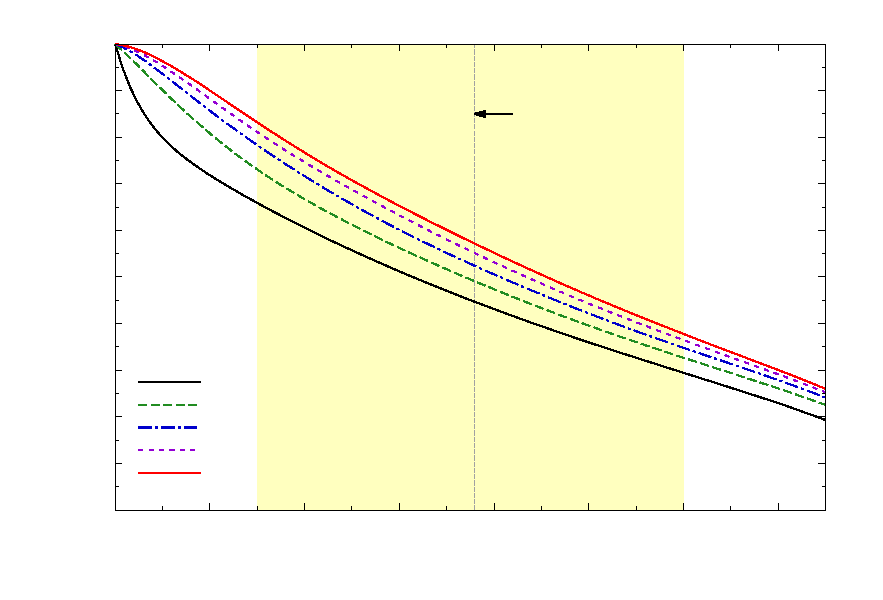
\includegraphics{plot_disp_wind_bess}}%
    \gplfronttext
  \end{picture}%
\endgroup

		}
	\end{figure}
\note[item]{
For example, the probability of power dispatched to the grid exceeding 0.38 p.u., corresponding to the capacity factor of the Snowtown wind farm (vertical dashed line), is 44.5\% with no energy storage (black solid curve), and rises to 52\% when coupled with a utility-scale battery with energy capacity of 0.50 p.u.\ (blue dot-dashed curve)
}	

\end{frame}

%%=========================================================================================%%
\begin{frame}
	\frametitle{Direction of future research}
	\framesubtitle{}

\note[item]{
A utility-scale, lithium-ion battery with energy capacity of 50 MWh is capable of supplying 25 MW for only two hours (based on battery specifications assumed for the virtual trials), and would cost in excess of USD 50 million.  Today, there are probably better, and more economical, renewable energy technologies for supplying baseload power, such as CST
}
\note[item]{
Powercor has invested AUD 8 million to install a lithium ion battery with 2 MWh capacity in Buninyong, Victoria.  It is designed to peak shave load on the distribution network and provide back-up power to 3,000 customers for one hour during a power outage
}
\note[item]{
Southern California Edison has invested USD 53 million to install a lithium ion battery with 32 MWh capacity.  It is testing the integration of the utility-scale battery into the electricity grid
}
\note[item]{
However, even within the bounds of current technology, we reckon that MPC could be implemented on a wind farm coupled with a utility-scale battery to serve some practical purpose
}	
	\begin{itemize}
		\item  Soaring wholesale electricity prices in SA during July 2016:
		\begin{itemize}
			\item  During the month RRP averaged \$229/MWh, more than three times the average price of any other region in the NEM
\note[item]{
There were three very large price spikes in SA that warranted investigation by AER, and they attributed the price spike on July 13 to wind forecast error
}
			\item  On 13 July 2016 electricity traded at \$7,068 during the 06:30 trading interval
			\item  AER reported ``[t]he major contributing factor to the high price was wind forecast error''
		\end{itemize}
		\item  Conjecture that if wind farms were to dependably supply power scheduled during pre-dispatch, then wholesale electricity prices would be less volatile and, on average, lower
		\item  Ongoing research proposal:
		\begin{itemize}
			\item  Extend incremental state-space model to a multi-period setting
			\item  Use pre-dispatch unconstrained intermittent generation forecasts (UIGF) produced by the Australian Wind Energy Forecasting System (AWEFS)
			\item  Empirically examine the dependability of supply of wind power scheduled during pre-dispatch --- up to 40 hours ahead of dispatch --- using battery energy storage to enable time shifting
		\end{itemize}
	\end{itemize}
	
	
\end{frame}

%%=========================================================================================%%
\end{document}

%%=========================================================================================%%
%%=========================================================================================%%
\begin{frame}
	\frametitle{<frame title>}
	\subframetitle{<subframe title>}

	<introductory statement>
	\begin{itemize}
		\item  <first item>
		\item  <more items>
	\end{itemize}
	
	\begin{figure}[!h]
	\centering
    	\label{fig:<label>}
	\scalebox{0.80}{
		\includegraphics{<file>}
		\input{<file>}
	}
	\end{figure}
	

\note[item]{
<notes>
}
\end{frame}

%%=========================================================================================%%


